\chapter{Project Management}


\section{Choice of Process Model}
A strict Scrum based approach to software development was required by the product owner in this project. In addition, the two principles \textit{decide as late as possible} and \textit{deliver as fast as possible}  from  LEAN software development were emphasised by the product owner. The development team had weekly meetings with the product owner and, thus, chose to structure the project in one-week long sprints. 

An agile approach to software development, coupled with short sprints were, in this project, essential to be able to accommodate the product owner's focus on the two Lean principles mentioned above. A more traditional plan-based approach would have forced both the customer and the development team to make decisions at a very early stage. 

Much of the communication between the product owner and the development team was based on pitching new ideas and solutions. This process relied heavily on mockups and wireframes, and the agile approach enabled us to easily present solutions at every stage of the development life cycle.


\subsection{Customer Meetings}
Every Thursday, the group met with the product owner for sprint retrospective and planning. During these meetings, the development team began with presenting a demo of the most recent version of the system to the product owner. Based on the feedback of the product owner, we settled on which features to keep, which to discard and which to develop further. This then lead us to the sprint planning of the next sprint, where we decided which features should be included in the next version of the product. 

The customer strongly practiced the Lean principle of \textit{decide as late as possible}, and this was an aspect of the development process unfamiliar to most of the team members. As the development team could not, form the start, neither rely on, nor elicit a fixed list of requirements, these weekly meetings were essential to prevent stagnation of the development. 

\subsection{Supervisor Meetings}
In addition to weekly meetings with the product owner for the development of the solution, the team also had bi-weekly meetings with our course supervisor, Soudabeh Khodambashi, to ensure our progress with the course as a whole. Prior to the meetings we submitted status reports to enable the supervisor to follow our progress and make her aware of any difficulties we might be experiencing. The status report gave a detailed overview of what we had done during the last meeting, what were our plans for the coming sprints, and any difficulties, coupled with an updated risk analysis.

\vspace{10mm}

//Should we include an example of a status report in the appendix? 
Ex: An example of a status report can be found in Appendix XX, figure XX.
% Status report link needed !

\section{Time Constraints and Work Breakdown Structure}

As stated in the course description, the workload of the course is expected to be approximately 20 hours per week. Thus, the group used this as a guiding estimate when calculating the time constraints of the project. We are 7 members on the team which led to 140 hours available each week, and taking into consideration holidays, we arrived at this estimate, Table \ref{table: Time}: 


\begin{table}[H]
\centering
\begin{tabu} to 0.8\textwidth{ |X[l]|X[l]|X[L]| } 
\hline \rowcolor{lightgray}
Months & Weeks & Hours  \\
\hline
Jan &  &  \\ 
\hline
Feb & 4 & 560\\ 
\hline
March & 3.5 & 490\\
\hline
April  & 4 & 560\\
\hline
May & 1 & 140\\
\hline
\textbf{Total} & & \textbf{1750}\\
\hline
\end{tabu}
\caption{Time Constraints}
\label{table: Time}
\end{table}

The groups were announced on Jan 21st, and the following week was spent meeting the group and having the initial customer meeting. Thus, no weeks in January were included in the time estimate of the project.
The term ends in April and, thus, only one week is allocated in May, primarily to finish up the report.

Following the initial meetings with the customer, the group decided on a work breakdown structure (WBS) for the project, see Figure \ref{fig:WBS}, and assigned percentages to the different sections. 
 
\begin{figure}[H]
\centering
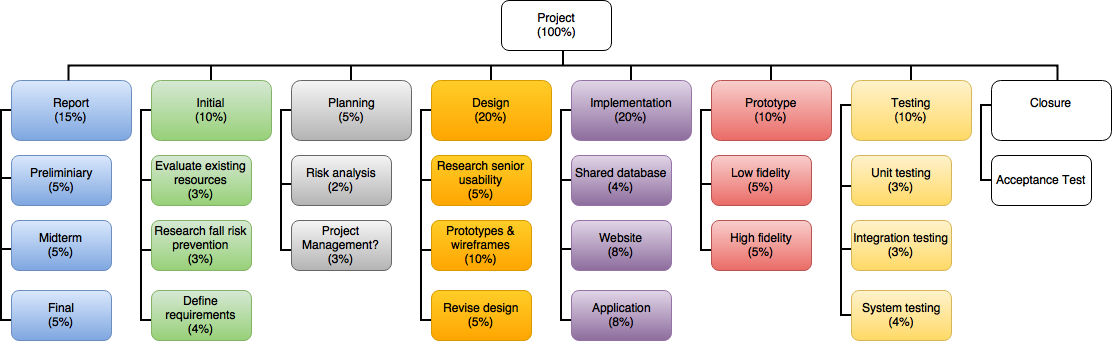
\includegraphics[scale=0.4]{Figures/WBS.png}
\caption{WBS}
\label{fig:WBS}
\end{figure}

Further, based on the WBS diagram and time constraints, we calculated how many hours we had available for each section which laid the foundation for project management. The allocation of hours on different aspects of the project can be seen in Table \ref{table: AllocatedTime}. 

\begin{table}[H]
\centering
\begin{tabu}{ |m{9em}|m{15em}|m{3em}|} 
\hline \rowcolor{lightgray}
Sections & Subsections & Hours\\
\hline
\multirow{3}{*}{Report 262.5h} & Preliminary & 87.5 \\

& Midterm & 87.5\\

& Final & 87.5\\
\hline
\multirow{3}{*}{Initial 175h} & Evaluate existing resources & 52.5\\
& Research fall risk prevention & 52.5\\
& Define requirements & 70\\
\hline
\multirow{2}{*}{Planning 87.5h} & Risk analysis & 35\\
& Project management & 52.5 \\
\hline
\multirow{3}{*}{Design 350h} & Research senior usability & 87.5\\
& Prototype and wireframes & 175\\
& Revise design & 175 \\
\hline
\multirow{3}{*}{Implementation 350h} & Shared database & 350\\
& Website & 140\\
& Application & 140 \\
\hline
\multirow{2}{*}{Prototype 175h} & Low fidelity & 175\\
& High fidelity & 175\\
\hline
\multirow{3}{*}{Testing 175h} & Unit testing & 52.5\\
& Integratiog testing & 52.5 \\
& System testing & 70 \\
\hline
\end{tabu}
\caption{Time allocated to different aspects of project}
\label{table: AllocatedTime}
\end{table}


\section{Risk Analysis}
Managing risk is essential to a software project and a meeting to analyse the risks was settled early. Firstly, in the \textit{risk identification} process, the team identified potential risks and organized them into several larger categories: requirements, team, planning and technical. Secondly, during \textit{risk analysis}, the team estimated both the likelihood and potential impact of each risk. This was done by awarding a number ranging from 1-9 where 1 indicates low likelihood and impact, and 9 indicates high likelihood and impact. Thirdly, the team identified actions to prevent and mitigate the risks during the \textit{risk planning} phase. The outcome of these three first phases is a risk assessment matrix, see Figure \ref{fig:RiskFull} in the appendix. The matrix lists all the risks accompanied by the likelihood and impact estimates along with preventative and mitigative actions. Below follows a condensed version of the risk assessment matrix, Figure \ref{fig:Risk}, giving a quick overview of how severe the different risks are, with R1, R2, R3, etc referring to Risk 1, Risk 2, Risk 3 and so on. The explanations of each risk can be found in the appendix, Figure \ref{fig:RiskFull}.
\begin{figure}[h!]
\centering
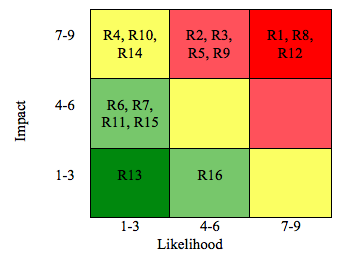
\includegraphics[scale=0.8]{Figures/RiskAnalysis.png}
\caption{Risk Analysis}
\label{fig:Risk}
\medskip
\small
R1, R2, R3, etc refers to Risk 1, Risk 2, Risk 3 and so forth, of the extended risk analysis matrix, see Figure \ref{fig:RiskFull} in the appendix.
\end{figure}

Lastly,  the team decided to perform \textit{risk monitoring} by regularly assessing the risks and revising the risk analysis matrix when needed. 


\section{Project Management Tools}
\subsection{GitHub}
In addition to the source code management provided by git, using gitHub lets us share the repository with all the team members while at the same time providing several project management features including backlog management, task management, sprint organization and easy communications with the customer. Having code and project management features in the same place eases collaboration as all team members then know where to look for new tasks, and the state of the product. We were not aware of all of these features of GitHub at the beginning of the project and, only towards the end of the project, did the team switch to using gitHub's project management features. 
\subsection{Trello}
Trello is a tool to help people collaborate and organizes your projects into boards. At a glance Trello shows you what is being worked on, who is working on what and what remains to be done. 
As we, as a team,  do not have office space or an alternative fixed location to work from, we do not have a suitable place for a physical Scrum board. Trello is  thus an online alternative to the Scum board which shows the current status for the project, or at least the sprint.
\subsection{Google Docs}
Google Drive is a file storage and synchronization service that allows users to store files in the cloud, share files, and edit documents, spreadsheets, and presentations with collaborators. It is essential for our team that everyone in the team has the same access to documents relating to the project, and are able to contribute to them.
\section{Group Communication Tools}
\subsection{Slack}
Slack is a cloud-based team collaboration tool used for communication through different chat rooms and channels. We use slack for communication within the team. Slack also has an app which gives you  instant notifications if a group member post anything in one of the channels. Thus, this communication tool is therefore more suitable than for instance email communications as it allows more instant communication. It is also better suited to this project than Facebook, as it allows us to structure our communication into different channels. 

\section{Deviations}

The concept refining phase took much longer time that the team had initially anticipated, with the result of coding being postponed. However, the long concept refining phase, was one of the main focus points of the customer in the early stages. This led to us having more sprints devoted to wireframing than was initially planned, and thus implementation was pushed back. The product owner, however, was pleased with this line of development of rapid prototyping and did not seem to be dissatisfied with the fact that coding was postponed. Consequently, we do not consider the project to be delayed as a result of the coding delay.
\\\\
We also encountered some difficulties with eliciting requirements from the product owner. It appeared to us that the product owner often focused on what was to be accomplished by the next sprint, and we found it difficult to settle on a long term plan. Thus, no milestones for the whole project were decided upon, nor did we settle on a release plan. It was made clear that user testing would be an integral part of the project, but although we had a meeting to plan the usability test, no dates were ever settled in this regard either. Thus, making a concrete time plan has been difficult. This issue is expanded on in Chapter \ref{lessons}. 
\\\\
Another deviation from the plan was related to our sprint management. Halfway into the project the product owner instructed us to switch to GitHub's issue list as a sprint backlog. Up to this point, we had been keeping track of our tasks using a spreadsheet in Google docs. The switch made it easier for the client to keep track of the tasks. He also stressed that it was important to keep the code close to the roadmap of the development process.

\section{Team Organization}
\subsection{Responsibilities}
All team members were part of coding and planning in the projects, but the following areas of responsibility were distributed among the team members:
\begin{itemize}
    \item[] \textbf{Emil S. Andersen:} Project leader, communication manager and documents manager
    \item[] \textbf{Christoffer Jahren:} Head of mobile division, responsible for developing the mobile version, both iOS and Android version of the app.
    \item[] \textbf{Eirik Wist:} Co-head of mobile division 
    \item[] \textbf{Sindre Berntsen:} Documentation and datamodelling 
    \item[] \textbf{Sarah Svedenbrog:} Scrum master and report
    \item[] \textbf{Brang Nu Bok Tong:} Webmaster: frontend and backend.
    \item[] \textbf{Alexander Foosnæs:} Test leader 
\end{itemize}
\subsection{Pair-Programming}
Although the team members were assigned tasks individually, pair-programming was used extensively. Most of the team members were unfamiliar with the frameworks we used in the project and the learning curve was steep. When one team members had learnt something, and another was going to do the same, the two often pair-programmed so that the time invested in learning by one team member could directly benefit another team members and, in turn, the team.

In addition to teaching other team members how to do certain tasks, pair-programming was also used for problem-solving. If one team member had been working a long time on a task and not succeeding in fulfilling it, he/she would often team up with another. Often problems were solved quickly in this way, and both team members involved benefited from the process.

\section{Sprints}
\subsection*{Sprint 1: Feb 5th - Feb 11th}
Table \ref{table: sprint1} is a summary of sprint 1. See Appendix \ref{sprint1} for complete breakdown of sprint 1. 

\begin{table}[H]

\begin{tabu} to 1.0\textwidth { | X[l] | X[l]| }
\hline\rowcolor{lightgray}
Objective of sprint & Summary of tasks completed\\
\hline
User story video & User story video\\
\hline
Wireframes of web solution & Wireframes of web solution\\
\hline
Wireframes of mobile application & Wireframes of mobile application\\
\hline
\end{tabu}
\caption{Summary of sprint 1}
\label{table: sprint1}
\end{table}


\subsection*{Sprint 2: Feb 11th -Feb 18th}
Table \ref{table: sprint2} is a summary of sprint 2. See Appendix \ref{sprint2} for complete breakdown of sprint 2. 
\begin{table}[H]
\begin{tabu} to 1.0\textwidth { | X[l] | X[l]| }
\hline\rowcolor{lightgray}
Objective of sprint & Summary of tasks completed\\
\hline
Senior usability research & Senior usability research\\
\hline
Fall prevention research & Fall prevention research\\
\hline
Evaluate existing solutions & Evaluate existing solutions\\
\hline
Elicit concrete requirements form customer & \\
\hline
\end{tabu}
\caption{Summary of sprint 2}
\label{table: sprint2}
\end{table}

Comments:  In this sprint, we begun having difficulties with eliciting clear requirements from the customer.


\subsection*{Sprint 3: Feb 18th - Feb 25th}
Table \ref{table: sprint3} is a summary of sprint 3. See Appendix \ref{sprint3} for complete breakdown of sprint 3. 
\begin{table}[H]
\begin{tabu} to 1.0\textwidth { | X[l] | X[l]| }
\hline\rowcolor{lightgray}
Objective of sprint & Summary of tasks completed\\
\hline
Revised user story film & Revised user story film\\
\hline
Revised mockups & Revised mockups\\
\hline
Research technologies & Research technologies\\
\hline
\end{tabu}
\caption{Summary of sprint 3}
\label{table: sprint3}
\end{table}

Comment: This sprint was largely concerned with revising the concept for the solution and much time was spent updating mockups and the user story film.

\subsection*{Sprint 4: Feb 25th - March 3rd}
Table \ref{table: sprint4} is a summary of sprint 4. See Appendix \ref{sprint4} for complete breakdown of sprint 4. 
\begin{table}[H]
\begin{tabu} to 1.0\textwidth { | X[l] | X[l]| }
\hline\rowcolor{lightgray}
Objective of sprint & Summary of tasks completed\\
\hline
Installation manual & Installation manual\\
\hline
Download app from webpage & Download app from webpage\\
\hline
Set up database & Set up database\\
\hline
Create user profile & Create user profile without form validation\\
\hline
\end{tabu}
\caption{Summary of sprint 4}
\label{table: sprint4}
\end{table}

\subsection*{Sprint 5: March 3rd - March 10th }
Table \ref{table: sprint5} is a summary of sprint 5. See Appendix \ref{sprint5} for complete breakdown of sprint 5. 
\begin{table}[H]
\begin{tabu} to 1.0\textwidth { | X[l] | X[l]| }
\hline\rowcolor{lightgray}
Objective of sprint & Summary of tasks completed\\
\hline
Flowchart for website & Flowchart for website\\
\hline
Download app from webpage & Link to app on website\\
\hline
Fill placeholders on homepage with actual information & Fill placeholders on homepage with actual information\\
\hline
\end{tabu}
\caption{Summary of sprint 5}
\label{table: sprint5}
\end{table}

Comment: The html page for downloading the app was implemented, but actually downloading an app was pushed to the next sprint.

\subsection*{Sprint 6: March 10th - March 17th}
Table \ref{table: sprint6} is a summary of sprint 6. See Appendix \ref{sprint6} for complete breakdown of sprint 6. 
\begin{table}[H]
\begin{tabu} to 1.0\textwidth { | X[l] | X[l]| }
\hline\rowcolor{lightgray}
Objective of sprint & Summary of tasks completed\\
\hline
State diagram of website & State diagram of website\\
\hline
Register new user & Register new user\\
\hline
Research dashboard component & Research dashboard and web usability for seniors\\
\hline
\end{tabu}
\caption{Summary of sprint 6}
\label{table: sprint6}
\end{table}

Comment: Much time was spent working on the report in this sprints. Thus, our objectives focused more on research than implementing functionality.

\subsection*{Sprint 7: March 17th - April 14th}
Table \ref{table: sprint7} is a summary of sprint 7. See Appendix \ref{sprint7} for complete breakdown of sprint 7. 
\begin{table}[H]
\begin{tabu} to 1.0\textwidth { | X[l] | X[l]| }
\hline\rowcolor{lightgray}
Objective of sprint & Summary of tasks completed\\
\hline
Creating and displaying events & Events added to the database\\
\hline
Algorithms for newsfeed & Algorithms for newsfeed\\
\hline
Searchbar & Searchbar designed\\
\hline
\end{tabu}
\caption{Summary of sprint 7}
\label{table: sprint7}
\end{table}

\textbf{Comment:} As this sprint began just before Easter, the actual work began after Easter, and in order to be able to meet the customer and have a status update, we let this sprint last approximately two weeks. 

With the unfamiliar technology, creating and displaying events took much longer time than expected, and the tasks related to it were further broken down in later sprints.
The same applies to the functionality of the search bar.


\subsection*{Sprint 8: April 14th - April 21st}


Switched to sprint management on GitHub

Table \ref{table: sprint8} is a summary of sprint 8. See Appendix \ref{sprint8} for complete breakdown of sprint 8. 
\begin{table}[H]
\begin{tabu} to 1.0\textwidth { | X[l] | X[l]| }
\hline\rowcolor{lightgray}
Objective of sprint & Summary of tasks completed\\
\hline
Accept/decline invitations to events & Accept/decline invitations to events\\
\hline
Filter and sort events & Filter and sort events\\
\hline
Internationalizing text & \\
\hline
\end{tabu}
\caption{Summary of sprint 8}
\label{table: sprint8}
\end{table}

\textbf{Comment:} Making the text internationalized was postponed until the next sprint since the group member who was assigned to it was unexpectedly absent.

\subsection*{Sprint 9: April 21st - April 28th}
Table \ref{table: sprint9} is a summary of sprint 9. See Appendix \ref{sprint9} for complete breakdown of sprint 9. 
\begin{table}[H]
\begin{tabu} to 1.0\textwidth { | X[l] | X[l]| }
\hline\rowcolor{lightgray}
Objective of sprint & Summary of tasks completed\\
\hline
Update event & Update event\\
\hline
Admin view & Admin view\\
\hline
Bug fixing & Bug fixing\\
\hline
\end{tabu}
\caption{Summary of sprint 9}
\label{table: sprint9}
\end{table}

\subsection*{Sprint 10: April 28th - May 6th }
Table \ref{table: sprint10} is a summary of sprint 10. See Appendix \ref{sprint10} for complete breakdown of sprint 10. 
\begin{table}[H]
\begin{tabu} to 1.0\textwidth { | X[l] | X[l]| }
\hline\rowcolor{lightgray}
Objective of sprint & Summary of tasks completed\\
\hline
App integration & fill in what got done\\
\hline
App roadmap & fill in what got done\\
\hline
\end{tabu}
\caption{Summary of sprint 10}
\label{table: sprint10}
\end{table}

\textbf{Comment:} We're currently in this sprint, so we will fill it out once we are done.

\section{Gantt Chart}
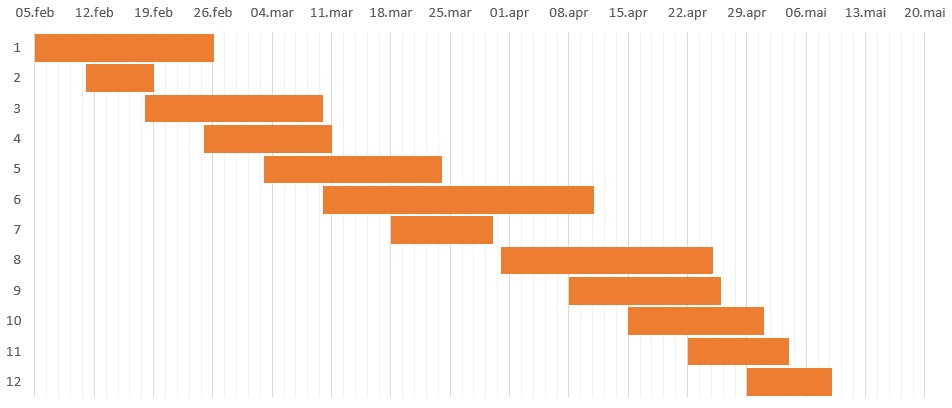
\includegraphics[width=1.0\textwidth]{Figures/Gantdiagram}

//The Gantt chart must be elaborated on here as an evaluation of all our sprints combined.